\documentclass[11pt,a4paper]{article}
\usepackage[margin=2.4cm]{geometry}
\usepackage[T1]{fontenc}
\usepackage{lmodern,microtype}
\usepackage{amsmath,amssymb,amsthm}
\usepackage{booktabs,graphicx,xcolor}
\usepackage[hidelinks]{hyperref}
\usepackage{enumitem}
\setlist{nosep,leftmargin=1.4em}
\setlength{\emergencystretch}{2.5em}
\newtheorem{proposition}{Proposition}
\usepackage{url,array}
\DeclareUrlCommand\code{\urlstyle{tt}}  % breaks at _ . /
\newcommand{\E}{\mathbb{E}}
\newcommand{\Var}{\mathrm{Var}}
\newcommand{\PhRevision}{a7371c5}
\newcommand{\PhVersion}{1.0.0.dev1}
\newcommand{\PhNumpy}{2.4.6}
\newcommand{\PhNumba}{0.66.0}
\newcommand{\PhMsprime}{1.4.2}
\newcommand{\PhPython}{3.14.6}
\newcommand{\PhMachine}{Darwin arm64}
\newcommand{\PhLoad}{11.5}
\newcommand{\PhSeconds}{116}
\newcommand{\PhPedN}{367}
\newcommand{\PhPedDraws}{2000}
\newcommand{\PhPedRms}{0.998}
\newcommand{\PhLambda}{1.002}
\newcommand{\PhLambdaSd}{0.061}
\newcommand{\PhEffectsErr}{1.1e-16}
\newcommand{\PhBgFree}{0.504}
\newcommand{\PhBgDense}{0.512}
\newcommand{\PhCoalSeeds}{30}
\newcommand{\PhCoalN}{100}
\newcommand{\PhCoalKb}{200}
\newcommand{\PhCoalMaxZ}{1.6}
\newcommand{\PhTraitSpeedup}{25}


\title{\textbf{phensim}: genotype, phenotype and summary-statistic\\
simulation for statistical genetics\\[0.4em]\large Technical report}
\author{phensim \PhVersion{} (revision \texttt{\PhRevision})}
\date{October 2026}

\begin{document}
\maketitle

\begin{abstract}
\noindent phensim is a NumPy-only Python package for simulating the data
that statistical-genetics methods are evaluated on. It covers genotypes with
realistic linkage disequilibrium (LD), phenotypes with known genetic
architecture, GWAS summary statistics under population LD, finite
reference panels, pedigrees and their relationship matrices, kinship
estimators and PLINK output. Every simulator is seeded, validates its
inputs, and returns its ground truth alongside the data.

The package contains a built-in, JIT-compiled implementation of Hudson's
coalescent with recombination. Across \PhCoalSeeds{} seeds it agrees with
msprime on site counts, nucleotide diversity and the decay of LD with
distance. The trait simulators draw the infinitesimal background from the
same scaled genomic relationship matrix a mixed model fits, through an
exact factor that never forms an $n\times n$ matrix. The
summary-statistic layer reproduces, bit for bit, the benchmark simulators
of the LDpred3 family that phensim now hosts.

We describe the models, the algorithms and the numerical contracts, and
report measured agreement between realized and target quantities together
with indicative costs.
\end{abstract}

\section{Introduction}
Simulation is how a statistical-genetics method earns trust before it
meets real data: only with a known truth can bias, calibration, power and
cost be measured. Methods that model LD (polygenic scores, fine-mapping,
heritability and genetic-correlation estimators) need simulators that get
LD, allele frequencies and the generating model right. Their
summary-statistic variants additionally need the regression-with-summary-statistics (RSS)
model~\cite{zhu2017} and realistic reference-panel noise.

phensim began as a teaching snippet. It grew into the shared simulator of
a family of packages (ldpred3, bipred, gwfm, g2gfun, multipgs, and the
pedigree code of ltpred) whose benchmark suites previously each carried
their own copies. It follows six design principles:
\begin{itemize}
\item \textbf{Model consistency.} Data are generated from the model an
  estimator fits: the infinitesimal background uses the same scaled GRM a
  mixed model uses, and summary statistics use the exact RSS likelihood.
\item \textbf{Truth returned.} Every simulator returns its generating
  components (background, QTL effects, causal sets, liabilities, the
  relationship matrix), so estimands can be scored exactly.
\item \textbf{Validated inputs.} Malformed inputs raise before any work is
  done or any file is written, rather than being coerced.
\item \textbf{Reproducibility.} Every function takes a seed or a NumPy
  \code{Generator}, and draw orders are documented contracts.
\item \textbf{Minimal dependencies.} The core needs only NumPy. Numba
  accelerates the coalescent; msprime is an optional second backend.
\item \textbf{Memory discipline.} Genotypes are \code{int8}, LD is
  validated in bounded tiles, and the large draws avoid $n\times n$ or
  genome-wide intermediates.
\end{itemize}

\section{Package overview}
Table~\ref{tab:api} lists the public API. All genotype simulators return
sample-major \code{int8} dosages in $\{0,1,2\}$ with columns in physical
order. LD is passed as a list of dense $(R, \mathit{ix})$ blocks that tile
the variants exactly once. Figure~\ref{fig:ld} contrasts the LD of the
three structured genotype models.

\begin{table}[ht]\centering\small
\caption{Public API by module.}\label{tab:api}
\begin{tabular}{p{2.1cm}>{\raggedright\arraybackslash}p{12.4cm}}
\toprule
Module & Functions \\
\midrule
genotypes & \code{simulate_independent}, \code{simulate_population_structure}, \code{simulate_ar1_blocks}, \code{realistic_block_sizes}, \code{simulate_haplotype_blocks}, \code{simulate_coalescent}, \code{simulate_by_mutation_rate} \\
phenotypes & \code{simulate_trait}, \code{simulate_binary_trait}, \code{simulate_confounded_trait}, \code{simulate_gxe_trait}, \code{simulate_correlated_traits}, \code{ascertain_case_control}, \code{h2_liability}, \code{n_eff_case_control} \\
sumstats & \code{simulate_effects}, \code{simulate_effects_pair}, \code{genetic_correlation}, \code{simulate_sumstats}, \code{simulate_sumstats_pair}, \code{shake_ld}, \code{prepare_blocks}, \code{gwas_scan} \\
pedigree & \code{simulate_pedigree}, \code{pedigree_birth_times}, \code{kinship_from_pedigree}, \code{mendelian_draw} \\
kinship & \code{grm}, \code{ibs_kinship}, \code{loco_kinships}, \code{iter_loco_kinships}, \code{windowed_kinships} \\
io & \code{write_plink} \\
\bottomrule
\end{tabular}
\end{table}

\begin{figure}[ht]\centering
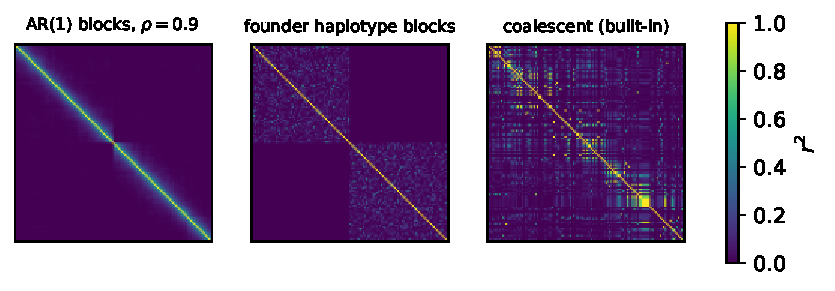
\includegraphics[width=\textwidth]{figures/ld_structure.pdf}
\caption{Squared correlation between 120 consecutive SNPs in 1000
simulated individuals. AR(1) blocks have smooth geometric decay and hard
block edges. Founder haplotype copying produces patchy haplotype sharing.
The coalescent produces recombination-driven, irregular LD whose block
boundaries are not imposed.}\label{fig:ld}
\end{figure}

\section{Genotype models}
\paragraph{Independent and structured SNPs.}
\code{simulate_independent} draws $G_{ij}\sim\mathrm{Bin}(2,p_j)$, where
$p_j$ is either a fixed minor allele frequency or drawn from a named
frequency spectrum (Beta, uniform, rare or common). Each site's minor
allele is the counted allele with probability $1/2$.

\code{simulate_population_structure} draws base frequencies
\[
p_j=\mathrm{clip}\big(\mathrm{maf}+N(0,0.05^2),\,0.05,\,0.95\big)
\]
and then, independently for each of $K$ populations, either the normal approximation
$p_{jk}\sim N(p_j,F p_j(1-p_j))$ or the exact Balding--Nichols
distribution~\cite{balding1995}
\[
p_{jk}\sim\mathrm{Beta}\Big(\tfrac{p_j(1-F)}{F},\tfrac{(1-p_j)(1-F)}{F}\Big),
\]
clipped to $[0.01,0.99]$.

\paragraph{AR(1) haplotype blocks.}
Within a block of $k$ SNPs, each individual carries two latent haplotypes
$z\sim N(0,C)$ with $C_{ij}=\rho^{|i-j|}$. A haplotype carries the allele
at SNP $j$ when $z_j>\Phi^{-1}(1-f_j)$, so the allele frequency is exactly
$f_j$; the dosage sums the two haplotypes. The default draws
$z=L\varepsilon$ with $LL^\top=C+10^{-8}I$. This is the family's historical
stream, which phensim reproduces bit for bit.
The alternative recursion
$z_j=\rho z_{j-1}+\sqrt{1-\rho^2}\,\varepsilon_j$ costs $O(nk)$, needs no
factorization, and is exact at $\rho=\pm1$. Both consume the same normals.
\code{realistic_block_sizes} draws log-normal block lengths with a
chosen coefficient of variation, which stresses the few large blocks that
dominate quadratic LD work.

\paragraph{Founder haplotype copying.}
Each block has a small set of Bernoulli(0.3) founder haplotypes. Every
individual copies two founders, with per-site flips at a mutation rate.
This gives genuine haplotype sharing at the cost of one pass.

\paragraph{Coalescent genotypes.}
\code{simulate_coalescent} grows a segment until at least $m$
SNPs pass the MAF filter. It starts at the larger of 1\,Mb and $m/1200$\,Mb
and multiplies the length by 1.8 per retry. It then keeps the first $m$
of those SNPs in physical order and cuts them into contiguous blocks. \code{simulate_by_mutation_rate}
instead fixes the segment and recombination rate, so the genealogy is
determined by the seed and the mutation rate alone controls SNP density.
This is the density lever used in the family's scaling benchmarks.

\section{The built-in coalescent engine}\label{sec:coal}
The engine is a compact implementation of Hudson's coalescent with
recombination~\cite{hudson1983} for one constant-size diploid population,
written to compile end to end under Numba. It writes dosages directly
instead of building a tree-sequence table collection.

\paragraph{Ancestry.}
The simulation starts from $2n$ haploid lineages carrying $[0,L)$. With
$k$ lineages, the next event occurs after an exponential waiting time at
total rate
\[
\lambda=\binom{k}{2}\frac{1}{2N_e}+r\sum_i\ell_i ,
\]
where $\ell_i$ is the distance between lineage $i$'s leftmost and
rightmost ancestral positions. A recombining lineage is chosen in
proportion to $\ell_i$ through a Fenwick tree~\cite{fenwick1994}, in
$O(\log k)$. The breakpoint is uniform on that span, gaps included, and is
clamped to the representable interior of the span.

Coalescence merges the two segment lists. Each overlapping interval
creates a node and two edges, and each segment carries the number of
samples below it. An interval whose count reaches $2n$ has found its most
recent common ancestor and leaves the simulation, which is what makes the
process terminate.

\paragraph{Mutations and genotypes.}
Each edge receives $\mathrm{Poisson}(\mu\,t_{\mathrm{branch}}\,\mathrm{span})$
infinite-sites mutations at uniform positions. Densification then sweeps
the marginal trees left to right, inserting edges by (left, parent time)
and removing them by (right, $-$parent time), as in tskit. Each mutation
adds one to every sample below its node, and haplotypes $2i$ and $2i+1$
form individual $i$.

\paragraph{Engineering.}
All work arrays are preallocated from expected event counts. On overflow
the engine doubles the buffer and reruns with the same seed, which
reproduces the same events, so a caller never sees a partial result. The
ancestry seed is the caller's seed masked to 31 bits, and the mutation
stream uses $(s\cdot2654435761)\bmod2^{31}$. The public functions accept
seeds in $[1,2^{31})$, the range both backends honour. Without Numba the
same code runs as pure Python on NumPy's global generator, whose state is
saved and restored around each call. Linked-list and Fenwick-weight
invariants are asserted at every event boundary in the test suite.

\paragraph{Agreement with msprime.}
msprime~\cite{kelleher2016,baumdicker2022} is the reference implementation;
phensim calls it on a continuous genome with the binary mutation model. We
simulated $n=\PhCoalN$ diploids on \PhCoalKb\,kb with
$N_e=10^4$ and $r=\mu=10^{-8}$, for \PhCoalSeeds{} seeds per backend.

Table~\ref{tab:coal} shows that site counts and nucleotide diversity agree
with each other and with the neutral expectations
$\E[S]=\theta\sum_{i<2n}1/i$ and $\E[\pi]=\theta$, where $\theta=4N_e\mu L$.
Figure~\ref{fig:decay} shows the decay of $r^2$ with physical distance:
in no distance bin do the backends differ by more than \PhCoalMaxZ{}
standard errors. These
are bounded distributional checks, not a proof of equivalence; the
backends draw different events from the same model.

\begin{table}[ht]\centering\small
\caption{Coalescent backends, mean over \PhCoalSeeds{} seeds (standard
error).}\label{tab:coal}
\begin{tabular}{lrr}
\toprule
Backend & Segregating sites (SE) & Diversity $\sum 2f(1-f)$ (SE) \\
\midrule
built-in (Numba) & 478 (9) & 82 (2) \\
msprime 1.4 & 477 (6) & 82 (2) \\
neutral expectation & 470 & 80 \\
\bottomrule
\end{tabular}

\end{table}

\begin{figure}[ht]\centering
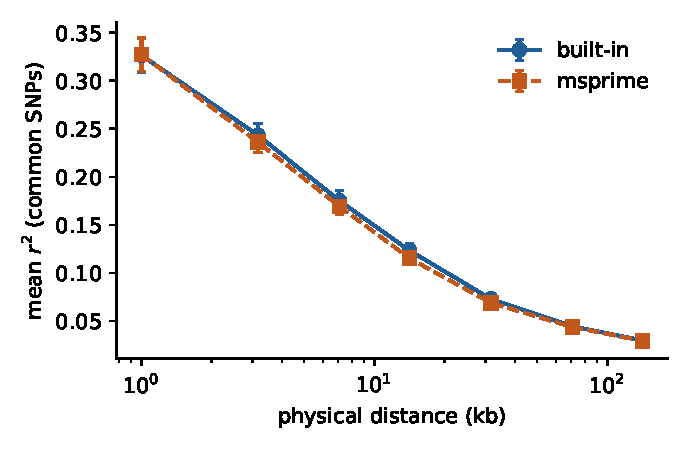
\includegraphics[width=0.62\textwidth]{figures/ld_decay.pdf}
\caption{Mean $r^2$ between common SNPs (MAF $\ge 0.05$) by physical
distance, for the built-in engine and msprime with the same design as
Table~\ref{tab:coal}. Bars are 95\% intervals over seeds.}\label{fig:decay}
\end{figure}

\section{Kinship}
\code{grm} standardizes each variant over its called samples (missing
calls contribute zero)~\cite{yang2010} and forms $ZZ^\top/m$. It then
applies the EMMAX scaling~\cite{kang2010}: subtract the mean off-diagonal
element, then divide by the mean diagonal.

Leave-one-chromosome-out matrices subtract each chromosome's Gram from the
full Gram under the same global standardization, so they are exact rather
than re-estimated. \code{windowed_kinships} splits the Gram the same way
into a local window and its complement. \code{ibs_kinship} is the per-pair
fraction of identical called genotypes, computed with one-hot GEMMs.

\section{Phenotype models}
\code{simulate_trait} builds $\ell=u+q+e$. The infinitesimal background
is $u\sim N(0,\sigma_u^2K)$, where $K$ is the scaled GRM a mixed model
would fit. The QTL component $q$ comes from causal variants, and the
residual is $e\sim N(0,1-h^2)$. Three architectures split $h^2$:
\code{mixed} gives half to $u$ and half to $q$, \code{infinitesimal} gives
all of it to $u$, and \code{qtl} gives all of it to $q$. QTL effects are
normal or of equal magnitude, act on standardized causal columns, and are
rescaled so that the in-sample $\Var(q)$ equals its target exactly.

\begin{proposition}[Matrix-free background]
Let $Z$ be the called-standardized genotypes, whose columns sum to zero,
and let $S=\sum_{ij}Z_{ij}^2$. The EMMAX-scaled GRM equals
$K=\frac{n-1}{S}ZZ^\top+\frac1nJ$. Hence
\[
u=\sigma_u\Big(\sqrt{\tfrac{n-1}{S}}\,Zw+\tfrac{c}{\sqrt n}\Big),
\qquad w\sim N(0,I_m),\ c\sim N(0,1),
\]
has covariance exactly $\sigma_u^2K$.
\end{proposition}
\begin{proof}
Write $K_0=ZZ^\top/m$. Its grand sum is $\mathbf1^\top Z Z^\top\mathbf1/m=0$
and its trace is $S/m$. The mean off-diagonal element is therefore
$-S/(mn(n-1))$. After subtracting it, the mean diagonal is $S/(m(n-1))$,
and dividing by it gives the stated $K$. The factor
$F=[\sqrt{(n-1)/S}\,Z,\ \mathbf1/\sqrt n]$ satisfies $FF^\top=K$.
\end{proof}
The draw therefore needs $m+1$ normals and one matrix--vector product,
with no $n\times n$ matrix and no eigendecomposition. Its in-sample
variance has expectation $\sigma_u^2(1-1/n)$, because $\mathbf1^\top
K\mathbf1=n$. A supplied $K$ is drawn through its eigendecomposition
instead, and the two give the same distribution: in
Table~\ref{tab:pheno} the background variances are \PhBgFree{} and
\PhBgDense{} against an expectation of $0.500$.

\paragraph{Derived traits.}
\begin{itemize}
\item \textbf{Binary traits} threshold the liability at
  $\Phi^{-1}(1-K)$.
\item \textbf{Confounded traits} add a share $s$ of variance along the
  leading eigenvector of $K$, the canonical population-structure axis,
  reusing the same eigendecomposition for the background.
\item \textbf{Gene--environment traits} add standardized causal genotypes
  multiplied by a standardized environment, scaled to the interaction
  variance.
\item \textbf{Correlated traits} share both components across traits:
  $g_b\propto r_gu_1+\sqrt{1-r_g^2}\,u_2+r_gq_1+\sqrt{1-r_g^2}\,q_2$.
  This targets the \emph{total} genetic correlation and is exact at
  $r_g=\pm1$.
\end{itemize}
\code{ascertain_case_control} samples exact case and control counts, and
\code{h2_liability} implements the observed-to-liability transformation
of Lee et al.~\cite{lee2011}. It warns unless the study case fraction is
given.

Table~\ref{tab:pheno} compares realized and target quantities over 40
draws on a coalescent panel of 1500 individuals and 3000 SNPs. Every
target is recovered within simulation error. The realized variance shares
are fractions of the realized liability variance, so they fluctuate with
the sample covariances between components.

\begin{table}[ht]\centering\small
\caption{Phenotype simulators: target versus realized. For
\texttt{simulate\_trait} the three numbers are the background, QTL and total
genetic shares of liability variance.}\label{tab:pheno}
\resizebox{\textwidth}{!}{\begin{tabular}{lll}
\toprule
Simulator and quantity & Target & Realized mean (SD), 40 draws \\
\midrule
\texttt{simulate\_trait} (mixed) & 0.25 / 0.25 / 0.50 & 0.25 (0.03) / 0.25 (0.02) / 0.50 (0.03) \\
\texttt{simulate\_trait} (infinitesimal) & 0.50 / 0.00 / 0.50 & 0.50 (0.04) / 0.00 (0.00) / 0.50 (0.04) \\
\texttt{simulate\_trait} (qtl) & 0.00 / 0.50 / 0.50 & 0.00 (0.00) / 0.51 (0.01) / 0.51 (0.01) \\
background variance, $K$ omitted / supplied & 0.500 & 0.504 (0.074) / 0.512 (0.081) \\
\texttt{simulate\_binary\_trait} prevalence & 0.05 & 0.049 (0.007) \\
\texttt{simulate\_binary\_trait} prevalence & 0.20 & 0.201 (0.012) \\
\texttt{simulate\_correlated\_traits} $r_g$ & 0.00 & -0.023 (0.136) \\
\texttt{simulate\_correlated\_traits} $r_g$ & 0.50 & 0.476 (0.095) \\
\texttt{simulate\_correlated\_traits} $r_g$ & 0.90 & 0.896 (0.016) \\
\texttt{simulate\_gxe\_trait} interaction share & 0.20 & 0.199 (0.012) \\
\bottomrule
\end{tabular}
}
\end{table}

\section{Summary statistics}
\paragraph{The RSS model.}
With standardized effects $\beta$ and block-diagonal population LD $R$,
marginal GWAS effects are drawn as~\cite{zhu2017}
\[
\hat\beta=R\beta+\varepsilon,\qquad\varepsilon\sim N(0,R/n),
\]
or $N(0,DRD)$ with $D_{jj}=n_j^{-1/2}$ for per-variant sample sizes. Each
block contributes $\varepsilon=Fz/\sqrt n$ with $z\sim N(0,I_r)$. The
factor $F$ is chosen per call:
\begin{itemize}
\item by default, the exact factor of $R$: Cholesky, or $V\Lambda^{1/2}$
  for singular LD, with no diagonal noise added;
\item with \code{jitter}, the Cholesky factor of $R+\epsilon I$;
\item with \code{factors}, matrices supplied by the caller, for example an
  eigenvalue-clipped root of thresholded LD, which need not be PSD.
\end{itemize}
The signal always uses $R$. \code{prepare_blocks} validates and factors
the blocks once into a read-only snapshot that every consumer accepts.

\paragraph{Effects.}
\code{simulate_effects} draws a sparse, polygenic, equal-magnitude or
MAF-dependent shape and rescales it so that $\beta^\top R\beta=h^2$
exactly. The MAF-dependent shape uses
$\beta_j\propto[2f_j(1-f_j)]^{(1+\alpha)/2}$, so the per-allele variance is
proportional to $[2f_j(1-f_j)]^{\alpha}$. This is the convention of
LDAK~\cite{speed2012}, SBayesS~\cite{zeng2018} and ldpred3, in which
$\alpha=-1$ means no MAF dependence.

\code{simulate_effects_pair} draws shared effects with correlation
$\rho$ and scales each trait to its own $h^2$. The causal layout is either
a shared Bernoulli($p$) set, or exact per-trait and shared counts
$(n_a,n_b,n_{ab})$; the latter is the bivariate causal mixture of
MiXeR~\cite{frei2019}, whose target genetic correlation is
$\rho\,n_{ab}/\sqrt{n_an_b}$. \code{genetic_correlation} returns the
correlation realized under the LD.

\paragraph{Two studies and reference panels.}
\code{simulate_sumstats_pair} draws $z_a$ and then $z_b$ per block and
sets $\varepsilon_b=F(\rho z_a+\sqrt{1-\rho^2}z_b)/\sqrt{n_b}$, which gives
cross-covariance $\rho R/\sqrt{n_an_b}$. Here $\rho$ is the
sampling-noise correlation, not the fraction of overlapping participants.

\code{shake_ld} simulates a reference panel: it draws $X=ZF^\top$ with
$n_{\mathrm{ref}}$ rows, standardizes the columns, and returns
$(1-s)X^\top X/n_{\mathrm{ref}}+sI$. An optional chunked path accumulates
the same draws with the stable one-pass update of Chan et
al.~\cite{chan1983}, bounding memory at $O(\mathrm{chunk}\cdot k+k^2)$.

\paragraph{Individual-level GWAS.}
\code{gwas_scan} fits each variant on its called samples. It reports the
Pearson correlation $r$, the standard error $\sqrt{(1-r^2)/(n-2)}$, the OLS
$t$ statistic and a normal $p$-value. A variant whose called genotypes or
called phenotypes are constant, tested exactly, returns NaN instead of a
roundoff statistic.

\paragraph{Validation tolerances.}
Blocks must tile the variants and be finite, symmetric, unit-diagonal,
bounded in $[-1,1]$ and PSD. Validation runs in tiles of 256 rows, so
genome-wide LD is never assembled. Tolerances follow the input precision:
the relative tolerance is $\max(10^{-7},4\epsilon)$, and negative
eigenvalues are clipped up to
$k\max(64\,\epsilon_{64}\max(1,\lambda_{\max}),\epsilon_{\mathrm{in}})$.
float32 LD, the family's usual storage, is therefore judged at float32
roundoff.

Table~\ref{tab:ss} confirms each property against its theoretical
expectation. The empirical noise covariance matches $R/n$ to the error
expected of a Wishart estimate. Panel noise matches the large-sample
standard deviation of a sample correlation,
$(1-\rho^2)/\sqrt{n_{\mathrm{ref}}}$. Null scans are calibrated: mean
$\lambda_{\mathrm{GC}}=\PhLambda$ (SD \PhLambdaSd{}) over 40 null
traits with 5\% missing calls.

\begin{table}[ht]\centering\small
\caption{Summary-statistic layer: properties versus expectation.}\label{tab:ss}
\resizebox{\textwidth}{!}{\begin{tabular}{lll}
\toprule
Check & Expected & Realized \\
\midrule
\texttt{simulate\_effects}: $|\beta^\top R\beta - h^2|$, 4 architectures & 0 & 1.1e-16 \\
\texttt{simulate\_sumstats}: $\|n\,\widehat{\mathrm{Cov}} - R\|_F/\|R\|_F$, 4000 draws & $\approx 0.096$ & 0.095 \\
\texttt{simulate\_sumstats\_pair}: noise correlation & 0.40 & 0.399 \\
\texttt{simulate\_effects\_pair}: mean realized $r_g$ (40/40 causal, 20 shared, $\rho=0.8$) & 0.40 & 0.395 (0.160) \\
\texttt{shake\_ld}: off-diagonal RMSE, $n_{\mathrm{ref}}=100$ & $\approx0.096$ & 0.097 \\
\texttt{shake\_ld}: off-diagonal RMSE, $n_{\mathrm{ref}}=500$ & $\approx0.043$ & 0.045 \\
\texttt{shake\_ld}: off-diagonal RMSE, $n_{\mathrm{ref}}=2500$ & $\approx0.019$ & 0.020 \\
\texttt{gwas\_scan}: $\lambda_{\mathrm{GC}}$, 40 null traits, 5\% missing calls & 1 & 1.002 (0.061) \\
\bottomrule
\end{tabular}
}
\end{table}

\paragraph{Parity with the family.}
With \code{jitter=1e-4}, per-trait sample sizes and \code{shrink}, these
functions reproduce byte for byte:
\begin{itemize}
\item ldpred3: \code{_metrics.sumstats} and \code{_realistic_ld.panel_genome};
\item bipred: \code{rg_architectures.sim_effects}, \code{sumstats_pair},
  \code{ref_panel} and \code{realized_rg}, and
  \code{mixer_overlap._sim_mixture}.
\end{itemize}
This was checked against the siblings' own source and is pinned by
verbatim oracles in \code{tests/test_family_parity.py}. A sibling can
therefore replace its local copy without changing any seeded result.

\section{Pedigrees}
\code{simulate_pedigree} produces multi-generation trio tables from
founder couples. Each couple has two to four children, and remarriage
produces half-siblings. \code{kinship_from_pedigree} orders individuals
parents first and fills the additive relationship matrix with Henderson's
tabular recursion~\cite{henderson1976}:
\[
A_{kj}=\tfrac12(A_{s_kj}+A_{d_kj}),\qquad A_{kk}=1+\tfrac12A_{s_kd_k},
\]
where unknown parents contribute zero. The cost is $O(n^2)$, and the result
is exactly symmetric and includes inbreeding.

\code{mendelian_draw} samples $a\sim N(0,A)$ in $O(n)$ storage:
$a_i=\sum_{p}a_p/2+\sqrt{w_i}z_i$, summing over known parents, with
$w_i=1-\sum_pA_{pp}/4$. This is the Mendelian sampling variance
$(1-(F_s+F_d)/2)/2$ when both parents are known. The required diagonals
come from a memoized pair recursion.

Over \PhPedDraws{} draws on a simulated \PhPedN-person pedigree, which
includes inbred individuals, the empirical covariance matched $A$ with a
standardized root-mean-square error of \PhPedRms{}; pure sampling noise
gives $1$. \code{pedigree_birth_times} assigns generation-coherent birth
years and rejects inconsistent pedigrees.

\section{Output}
\code{write_plink} writes SNP-major PLINK~1 binary files. Genotypes are
coded 00, 10 and 11 for zero, one and two copies of BIM allele~2, with 01
for missing, packed four samples per byte. Every genotype and metadata
check, including unique and printable sample identifiers, PLINK chromosome
codes and integral positions, completes before any file is opened.

\section{Performance}
Table~\ref{tab:time} gives indicative single-thread costs. These were
measured on a shared machine (\PhMachine, load average \PhLoad), so
absolute numbers will vary; the comparisons are what matter.
\begin{itemize}
\item At this size the msprime backend is somewhat faster than the
  built-in engine. The built-in engine's value is that it has no compiled
  dependency and writes genotypes directly.
\item The matrix-free trait draw is about \PhTraitSpeedup{} times faster
  than drawing through a supplied $K$. The gap widens with $n$, because the
  eigendecomposition costs $O(n^3)$ while the matrix-free draw costs $O(nm)$.
\item Prepared LD blocks remove the per-call validation and factorization,
  which dominate repeated summary-statistic draws.
\item The AR(1) recursion is not faster at a block size of 200; it
  matters for very large blocks and exact $\rho=\pm1$.
\end{itemize}

\begin{table}[ht]\centering\small
\caption{Indicative wall-clock cost, median of three runs after a warm-up,
BLAS pinned to one thread.}\label{tab:time}
\begin{tabular}{lr}
\toprule
Call & Seconds (median of 3) \\
\midrule
simulate\_coalescent, $n=1000$, $m=10^4$, built-in & 0.73 \\
simulate\_coalescent, $n=1000$, $m=10^4$, msprime & 0.47 \\
simulate\_ar1\_blocks, $n=5000$, $m=2\times10^4$, Cholesky & 2.51 \\
simulate\_ar1\_blocks, $n=5000$, $m=2\times10^4$, scan & 3.51 \\
simulate\_trait, $n=3000$, $m=5000$, $K$ omitted (matrix-free) & 0.22 \\
simulate\_trait, $n=3000$, $m=5000$, $K$ supplied (eigh) & 5.37 \\
grm, $n=3000$, $m=5000$ & 0.43 \\
simulate\_sumstats, $m=5\times10^4$ (250 blocks of 200), raw blocks & 0.15 \\
simulate\_sumstats, same, prepared blocks & 0.01 \\
shake\_ld, same, $n_{\mathrm{ref}}=500$ & 0.29 \\
\bottomrule
\end{tabular}

\end{table}

\section{Reproducibility and integration}
\paragraph{Seeds.}
Seeds are integers, \code{None}, or NumPy \code{Generator}s. A
\code{Generator} continues its stream, so composed simulations remain
reproducible.

\paragraph{Draw orders.}
Draw orders are part of the contract, and every change to a seeded output
is recorded in the changelog. Results should carry the package version
and git revision. This report's own provenance is phensim \PhVersion{} at
revision \texttt{\PhRevision}, with NumPy \PhNumpy, Numba \PhNumba,
msprime \PhMsprime{} and Python \PhPython.

\paragraph{Sibling caches.}
Sibling repositories bind their caches to phensim's source:
\begin{itemize}
\item bipred tags cached coalescent segments with a hash of the coalescent,
  genotype and JIT modules, plus a hand-bumped msprime tag;
\item gwfm fingerprints the same files in its simulation cache;
\item ldpred3 records a hash of every phensim module in its run archives.
\end{itemize}
New features that do not touch genotypes therefore live outside those
modules. As a further consequence, a change to the coalescent or to the
msprime call invalidates downstream caches. Only some of these caches are
keyed automatically: in ldpred3, a cache version must be bumped by hand.

\section{Limitations and roadmap}
\paragraph{Limitations.}
\begin{itemize}
\item The coalescent models a single constant-size population, with no
  demography, migration or selection; msprime should be used directly for
  those.
\item Block models have no LD across block boundaries.
\item The prevalence target is exact only for Gaussian liabilities.
\item The RSS oracle assumes a single homogeneous sample.
\end{itemize}

\paragraph{Roadmap.}
A survey of the family identified further shared simulators worth
consolidating:
\begin{itemize}
\item register follow-up records with age of onset, competing mortality
  and censoring (ltpred, aadgen);
\item the exact LD of the AR(1) threshold model (aadgen);
\item public Balding--Nichols frequency draws and admixture (ppb, PLDSC);
\item a genome of independent coalescent blocks (eleven call sites).
\end{itemize}

\section*{Reproducing this report}
\begin{verbatim}
OPENBLAS_NUM_THREADS=1 OMP_NUM_THREADS=1 python report/make_evidence.py
cd report && tectonic phensim_report.tex
\end{verbatim}
The evidence script is fully seeded. It regenerates every table, figure and
quoted number, and took \PhSeconds\,s on the recording machine.

\begin{thebibliography}{99}\small
\bibitem{balding1995} D.~J.~Balding and R.~A.~Nichols. A method for quantifying differentiation between populations at multi-allelic loci and its implications for investigating identity and paternity. \emph{Genetica} 96:3--12, 1995.
\bibitem{baumdicker2022} F.~Baumdicker et al. Efficient ancestry and mutation simulation with msprime 1.0. \emph{Genetics} 220:iyab229, 2022.
\bibitem{chan1983} T.~F.~Chan, G.~H.~Golub and R.~J.~LeVeque. Algorithms for computing the sample variance: analysis and recommendations. \emph{The American Statistician} 37:242--247, 1983.
\bibitem{fenwick1994} P.~M.~Fenwick. A new data structure for cumulative frequency tables. \emph{Software: Practice and Experience} 24:327--336, 1994.
\bibitem{frei2019} O.~Frei et al. Bivariate causal mixture model quantifies polygenic overlap between complex traits beyond genetic correlation. \emph{Nature Communications} 10:2417, 2019.
\bibitem{henderson1976} C.~R.~Henderson. A simple method for computing the inverse of a numerator relationship matrix used in prediction of breeding values. \emph{Biometrics} 32:69--83, 1976.
\bibitem{hudson1983} R.~R.~Hudson. Properties of a neutral allele model with intragenic recombination. \emph{Theoretical Population Biology} 23:183--201, 1983.
\bibitem{kang2010} H.~M.~Kang et al. Variance component model to account for sample structure in genome-wide association studies. \emph{Nature Genetics} 42:348--354, 2010.
\bibitem{kelleher2016} J.~Kelleher, A.~M.~Etheridge and G.~McVean. Efficient coalescent simulation and genealogical analysis for large sample sizes. \emph{PLoS Computational Biology} 12:e1004842, 2016.
\bibitem{lee2011} S.~H.~Lee, N.~R.~Wray, M.~E.~Goddard and P.~M.~Visscher. Estimating missing heritability for disease from genome-wide association studies. \emph{American Journal of Human Genetics} 88:294--305, 2011.
\bibitem{speed2012} D.~Speed, G.~Hemani, M.~R.~Johnson and D.~J.~Balding. Improved heritability estimation from genome-wide SNPs. \emph{American Journal of Human Genetics} 91:1011--1021, 2012.
\bibitem{yang2010} J.~Yang et al. Common SNPs explain a large proportion of the heritability for human height. \emph{Nature Genetics} 42:565--569, 2010.
\bibitem{zeng2018} J.~Zeng et al. Signatures of negative selection in the genetic architecture of human complex traits. \emph{Nature Genetics} 50:746--753, 2018.
\bibitem{zhu2017} X.~Zhu and M.~Stephens. Bayesian large-scale multiple regression with summary statistics from genome-wide association studies. \emph{Annals of Applied Statistics} 11:1561--1592, 2017.
\end{thebibliography}
\end{document}
